\documentclass[10pt,twocolumn,letterpaper]{article}

\usepackage{cvpr}
\usepackage{times}
\usepackage{epsfig}
\usepackage{graphicx}
\usepackage{amsmath}
\usepackage{amssymb}

% Include other packages here, before hyperref.

% If you comment hyperref and then uncomment it, you should delete
% egpaper.aux before re-running latex.  (Or just hit 'q' on the first latex
% run, let it finish, and you should be clear).
\usepackage[breaklinks=true,bookmarks=false]{hyperref}

\cvprfinalcopy % *** Uncomment this line for the final submission

\def\cvprPaperID{****} % *** Enter the CVPR Paper ID here
\def\httilde{\mbox{\tt\raisebox{-.5ex}{\symbol{126}}}}

% Pages are numbered in submission mode, and unnumbered in camera-ready
%\ifcvprfinal\pagestyle{empty}\fi
\setcounter{page}{1}
\begin{document}

%%%%%%%%% TITLE
\title{COMS W4995 Project Milestone: Automatic Data Augmentation Policy Selection}

\author{Jonathan D. Armstrong\\
{\tt\small jda2160@columbia.edu}
% For a paper whose authors are all at the same institution,
% omit the following lines up until the closing ``}''.
% Additional authors and addresses can be added with ``\and'',
% just like the second author.
% To save space, use either the email address or home page, not both
\and
Jesse Galef\\
{\tt\small jbg2160@columbia.edu}
\and
Kyle Matoba\\
{\tt\small km3227@columbia.edu}
}

\maketitle
%\thispagestyle{empty}

%%%%%%%%% ABSTRACT
% \begin{abstract}
% \end{abstract}

% Evaluation metrics for project milestone (20 points)
% Introduction: 2 points
% Related work and references: 2 points
% Problem formulation, technical depth and innovation: 3 points
% Methods, technical depth and innovation, architecture and design: 5 points
% Preliminary results, Github repository, data, code correctness and readability: 8 points
 
%%%%%%%%% BODY TEXT
\section{Introduction}

% \cite{Real2018} 

\section{Related works}
The professor (I believe) mentioned in our first project meeting that data augmentation is indispensable in achieving state of the art performance in image classification. This makes sense, augmentation is achieved through sensible tweaks of the raw data -- it is easy to see why it \emph{should} work -- and it can be researched and tested independently of the architecture it is used to finally train. The Professor's statement seems to have been supported in our subsequent research. One compelling finding to this effect is that \cite{Recht2018} find that out of more than 20 models they entertained, the best-performing model on the CIFAR-10 dataset (\cite{Krizhevsk2009}) was a cutout (\cite{Devries2017}) regularised ``shake-shake'' architecture (\cite{Gastaldi2017}). Cutout is a data augmentation method which appends to the base data set additional occluded images that have had had contiguous regions set to ``zero'' (assuming the data has been normalised around this value). For example, in \autoref{fig:cutout}, we show a cutout region in a CIFAR 10 image of an ostrich.

\begin{figure}[t]
\begin{center}
   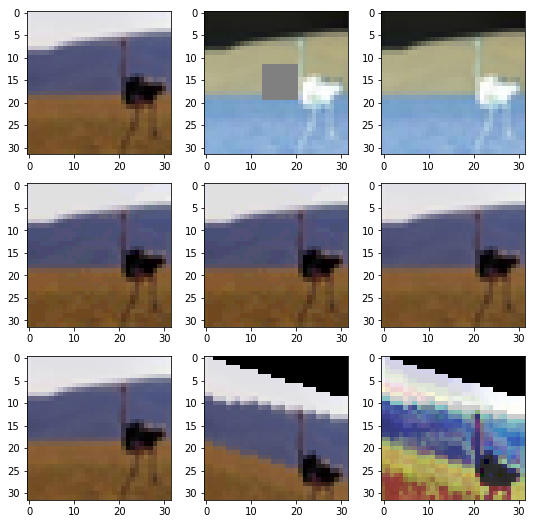
\includegraphics[trim={6.5cm 12.5cm 6.5cm 0}, clip, width=0.8\linewidth]{image.png}
% <left> <lower> <right> <upper>
\end{center}
   \caption{A ``cutout`` Bird}
\label{fig:cutout}
\end{figure}

% \pagebreak

Probably more importantly, not only was this model best in test-set accuracy, but it was also best on the newly-collected, truly out of sample dataset that is the innovation of \cite{Recht2018}. And further even to this, the drop between test set and truly out of sample performance was lower than for every other model -- the cutout-regularised shake-shake model was just barely the best on the test set, but was clearly a lot better of sample. The other well-performing cutout-regularised model, a wide resnet (\cite{Zagoruyko2016}), whilst beaten by some un-augmented models (though the shake-shake model itself has a straightforward interpretation as data augmentation applied to an representation), both in (test) and out of sample, sees a smaller dropoff between CIFAR 10 test and CIFAR10.1 data sets. 

This is intuitive enough, it one thinks that -- all else equal -- more regularised models should generalised better. 

\textbf{We need some discussion of reinforcement learning, I guess.}
% Happily google drive will continue run even when the space is fully taken up by 

\section{Preliminary results}

If there is one thing I have learned from many years of working data and modelling, it is to solve the apparently simple problems first, because usually they are not as easy as they appear, and often the entire project may turn out to be rethought (multiple times!). % I usually tell the younger members of my team that 80\% of the work is done in the last 20\% of the time, following a lot of set up. 
And even on the rare occasion that the easy bits end up being as straightforward as one expects, they often inform the hard bit importantly.
That is very much the approach I have taken thus far: I have been working to spec things out and generally understand all of the moving parts, especially the computational ones. 
% In my mind, it's better an unsuccessful at improving the state of the art project that runs, is correct, and can be meaninfully and completely analysed, than one which seems to do better on some simplified version of the problem, but we still aren't 100% certain that it runs correctly, and we've not managed to test it on the genuine out of sample data set, etc.

This is a project on meta learning, where we are working on the bleeding edge of performance on a , so  some of our work has unavoidably dealt with 

% My results have been slowed somewhat by the necessity of learning to use TensorFlow on an industrial scale, for example I took many hours to pick up TensorBoard. 

\section{Replicating \cite{Cubuk2018}}
A 

I have also checked the the ``CIFAR 10.1'' dataset\footnote{\url{https://github.com/modestyachts/CIFAR-10.1}}


\footnote{\url{https://cloud.google.com/tpu/docs/pricing}}

\subsection{Hardware Accelerators: GPUs and TPUs}
\cite{Cubuk2018} was a product of Google Brain, and while it does not demand hundreds of GPU-years to replicate, it (like most deep learning papers, I am beginning to learn) does entail significant computation. For even the least-demanding model, a complete fit would have taken about two months on my CPU. By changing it to running on the 

Unfortunately, moving from running tensorflow code from GPUs to TPUs is much less straightforward from moving from CPUs to GPUs). I have been refactoring the existing code to 


\section{Link to Github}
Currently the work is spread across a few repos, as well as Google Colab notebooks. We will work to consolidate things into a single, cleanly-runnable shape as we approach conclusion.

\begin{itemize}
\item \url{https://github.com/kylematoba/deeplearning-project}
\item \url{https://github.com/kylematoba/models}
\item \url{https://colab.research.google.com/drive/1qV3vCsjnEcm5a8nRpN40n4qgVKKBzBkd#scrollTo=uiht7wpPPPCP} (also checked into the \texttt{deeplearning-project} repo above)
\end{itemize}

% Note that we've not made the repo public, but we have permissioned \texttt{id2305@columbia.edu}, \texttt{id2303@columbia.edu}, \texttt{}

\nocite{Torralba2008}
{\small
\bibliographystyle{ieee}
\bibliography{../biblio}
}

\end{document}

